\nsection{Sierpinski Squares}

See also~:
\wwwurl{en.wikipedia.org/wiki/Sierpinski_triangle}

The Sierpinski triangle has the overall shape of an equilateral 
triangle, recursively subdivded into four smaller triangles~:
\begin{center}
\centering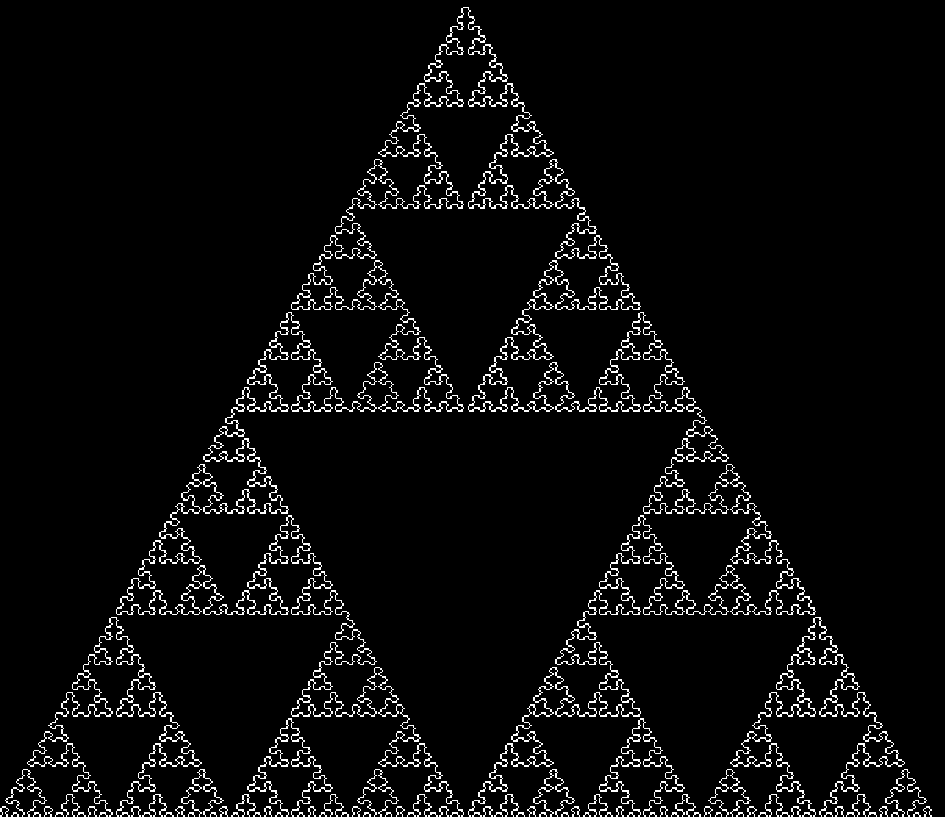
\includegraphics[scale=0.30]{./sierpinsky_curve.pdf}
\end{center}

However, we can approximate it by recursively drawing a square
as three smaller squares, as show below~:
\begin{center}
\centering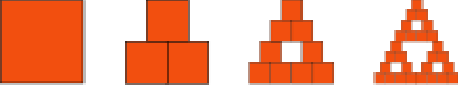
\includegraphics{./sierpinsky_squares.pdf}
\end{center}

The recursion should terminate when the squares are too small to draw with any more detail (e.g. one pixel, or one character in size).

\begin{exercise}
Write a program that, in plain text, produces a Sierpinski Triangle.
\end{exercise}

\begin{exercise}
Write a program that, using \verb^neillsimplescreen^,
produces a Sierpinski Triangle.
\end{exercise}

\begin{exercise}
Write a program that, using SDL, produces a Sierpinski Triangle.
\end{exercise}

